The image caption generation task is at the cross-section between Computer Vision (CV) and Natural Language Processing (NLP). It requires the computer to understand a visual scene and describe it into a grammatically correct natural sentence. Practical use cases vary from automated describing of images to visually impaired people \cite{mazzoni_2019} to context based image retrieval.

Show Attend and Tell (S.A.T.) proposed by \citeauthor{xu2016show} is an end-to-end deep learning approach that tries to solve the image caption generation problem. It combines an attention mechanism with LSTM to generate sentences that describe the given image. An example output from S.A.T can be seen in figure \ref{sat_example} Achieving good BLEU scores on Flickr8K, Flickr30K\cite{Flickr8k} and COCO\cite{lin2015microsoft} datasets. Although the scores are not state-of-the-art\cite{DBLP:journals/corr/abs-2107-06912} anymore. This model is chosen because it is small and thus can be run locally, and has publicly available implementations \cite{sgrvinod}.

\begin{figure*}[ht]
    \centering
    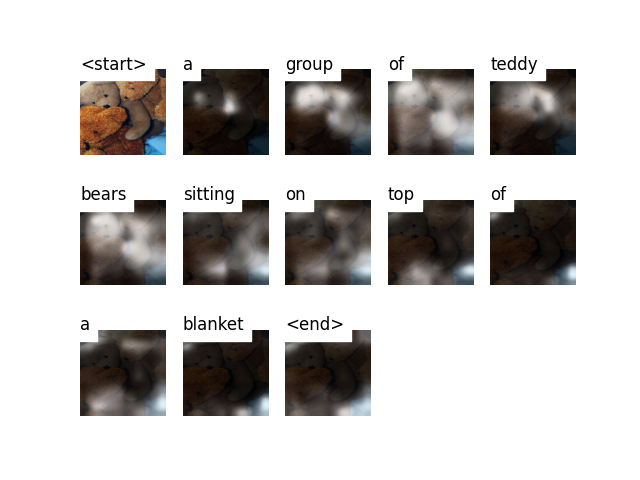
\includegraphics[width=0.9\textwidth]{figures/caption_teddy_normal.png} % first figure itself
    \caption{Prediction by Show Attend and Tell on a clean image. \newline Top left picture is the input image. The highlighted areas in white are the visualization of the attention per predicted word.}
    \label{sat_example}
\end{figure*}

Machine learning models can be very susceptible to noise where small changes to the input can lead to radically different outcomes. As shown by \citeauthor{goodfellow2015explaining} adding a specific (small) noise layer to an image can alter a correct prediction to a very confident wrong prediction. As can be seen in figure \ref{adv_gibbon}. Because the generation of the adversarial examples is not that computational expansive, they can be generated during training making the model more robust. It is also shown that these adversarial examples act as regularizes during training. Reducing the change of overfitting. \citeauthor{Kurakin} expands on generating adversarial examples showing that one can also steer the model towards a specific classification.

\begin{figure*}[h]
    \centering
    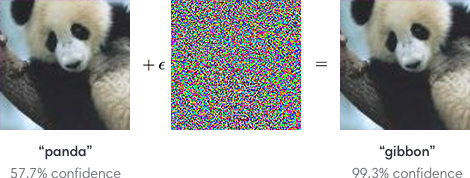
\includegraphics[width=0.9\textwidth]{figures/adversarial_img_1.png}
    \caption{Adversarial noise example from \protect\cite{goodfellow2015explaining}. Where $\epsilon=0.07$.}
    \label{adv_gibbon}
\end{figure*}

Combining these previous findings, S.A.T. can be used to find adversarial examples for image captioning models. These adversarial images can then be used to either improve current datasets by providing hard samples, or in a more malicious way. The latter being especially true when one can specify the output sentence for which an adversarial sample should be created. An additional benefit to adversarial samples that can be cheaply generated is that they can be generated during training of models and act as regularizes. Improving the robustness of the model. However, this is only viable if generating the adversarial samples is not computational expensive. Another point that makes S.A.T. an interesting target, is that it uses explicit attention to generate captions. Although attention has been surpassed by the use of transformers, it is still interesting to see if it is a potential attack vector in an adversarial setting.

\subsection{Motivation and Related Work}
In the last few years research in the direction of generating adversarial samples for gradient based models has been published \cite{goodfellow2015explaining,Kurakin} as well as research showing the usefulness of such adversarial samples\cite{Ilyas2019features}. The latter stating: "Adversarial vulnerability is a direct result of our models' sensitivity to well-generalizing features in the data." However, these generalizing features are only true for most samples, as models are optimized to do well in the average case. Inserting adversarial examples in training help regularize these non-robust features\cite{https://doi.org/10.48550/arxiv.1611.01236}. The Fast Gradient Sign Method was originally designed for classification task, however it (and variations) have been successfully adopted to other tasks such as object detection \cite{AdversarialAttacksOnFace,AdversarialFasterRCNN,DBLP:journals/corr/abs-1907-10310}, and most notably for this research on image captioning\cite{Hongge}. \citeauthor{Hongge}'s method Show-and-Fool successfully and robustly is able to attack Show-and-Tell\cite{showandtell} (predecessor of Show Attend and Tell). Achieving a success rate of 95.8\%, this does come at the cost of taking about 38 seconds to generate a single adversarial sample.

\subsubsection*{Adversarial Methods}
Over the last few years variations of the Fast Gradient Sign Method by \cite{goodfellow2015explaining} have been designed. The Iterative Fast Gradient Method by \citeauthor{Kurakin} applies the Fast Gradient Sign Method multiple times. Which is further improved by using various optimization techniques such as momentum \cite{9237700}, and in the case of Show-and-Fool the well known Adam\cite{kingma2017adam} optimizer. \citeauthor{EvaluatingRobustness} also directly include a distance metric in their adversarial optimization instead of clipping. Although very powerful techniques they are also computationally expensive and due to the computational limitations of this bachelor project, not feasible to apply extensively. Moreover, in the case of purely deceiving S.A.T. it is shown that classical Fast Gradient Sign Method already provides significant results.

\subsection{Research Questions}
This research investigates the susceptibility of S.A.T. against adversarial samples that are visually close but generate completely different descriptions as output. \citeauthor{Hongge} shows that Show-and-Tell is susceptible to adversarial samples, the question then arises if the attention added in S.A.T. makes it harder to generate adversarial samples. However, the attention mechanism might also be a new attack vector. If the attention is not focusing on the important parts of the image for generating the caption, the model is blind to those parts. It is therefore interesting to investigate if the attention can be used against S.A.T.
Concretely this paper will try to answer the following questions:.
\begin{itemize}
    \item Is S.A.T. susceptible to adversarial attacks using the Fast Gradient Sign Method?
    \item Can the attention of S.A.T. be abused by adversarial samples?
\end{itemize}
